\documentclass[a4paper, 12pt]{article}
\usepackage[a4paper,top=1.5cm, bottom=1.5cm, left=1cm, right=1cm]{geometry}

% Работа с русским языком
\usepackage[utf8]{inputenc}
\usepackage{mathtext}                % русские буквы в формулах
\usepackage[english, russian]{babel} % локализация и переносы

\usepackage{graphicx}   % Вставка изображений
\usepackage{float}      % "Плавающие" изображения3
\usepackage{wrapfig}    % Обтекание фигур (таблиц, картинок и прочего)
\usepackage{subfig}
\graphicspath{ {./images/} }

\usepackage{tabularx}
\usepackage{multirow}
\usepackage{amsmath}
\usepackage{amsfonts}
\usepackage{indentfirst}
\usepackage{longtable}
\graphicspath{{pictures/}}
\usepackage{natbib}
\usepackage{bm}

%%% Колонтитулы
\usepackage{titleps}
\newpagestyle{main}{
	\setheadrule{0.4pt}
	\sethead{Изучение плазмы газового разряда в неоне}{}{}
	\setfootrule{0.4pt}                       
	\setfoot{ФРКТ МФТИ, 2023}{}{\thepage} 
}
\pagestyle{main}  

\begin{document}
    \begin{titlepage}
	\begin{center}
            {\large МОСКОВСКИЙ ФИЗИКО-ТЕХНИЧЕСКИЙ ИНСТИТУТ (НАЦИОНАЛЬНЫЙ ИССЛЕДОВАТЕЛЬСКИЙ УНИВЕРСИТЕТ)}
	\end{center}
 
	\begin{center}
		{\large Физтех-школа радиотехники и компьютерных технологий}
	\end{center}
	
	\vspace{8cm}
	{\LARGE
		\begin{center}
                {\bf Отчёт о выполнении лабораторной работы 3.5.1}\\
                Изучение плазмы газового разряда в неоне
		\end{center}
	}
	\vspace{5cm}
	\begin{flushright}
		{\Large Автор:\\ Тихонов Дмитрий Романович, \\
			\vspace{0.2cm}
			студент группы Б01-206}
	\end{flushright}
	\vspace{5cm}
	\begin{center}
		\Large Долгопрудный, 2023
	\end{center}
    \end{titlepage}


    \section{Введение}

    \noindent \textbf{Цель работы:} изучение вольт-амперной характеристики тлеющего разряда; изучение свойств плазмы методом зондовых характеристик. \\

    \noindent \textbf{В работе используются:} стеклянная газоразрядная трубка, наполненная неоном; высоковольтный источник питания; источник питания постоянного тока; делитель напряжения; потенциометр; амперметры; вольтметры; переключатели.
    
    \section{Теоретические сведения}

    \textit{Двойным зондом} назывется система, состоящая их двух одинаковых зондов, расположенных на небольшом расстоянии друг от друга. Между зондами создаётся разность потенциалов $U$, которая по велиине много меньше плавающего потенциала: $\left|U\right|\ll\left|U_f\right|$. При этом оба зонда имеют относительно плазмы близкий к плавающему отрицательный потенциал, т.е. находятся на \textit{ионной} ветви вольт-амперной характеристики.

    При отсутствии разности потенциалов ток между зондами равен нулю. Рассчитаем величину тока, проходящего через двойной зонд вблизи точки $I = 0$. При небольших разностях потенциалов ионные токи на оба зонда равны ионному току насыщения и компенсируют друг друга. Величина результирующего тока целиком связана с различием в электронных токах. Пусть потенциал на первом зонде равен\[U_1 = U_f + \Delta U_1,\] а на втором \[U_2=U_f+\Delta U_2.\] Предполагается, что $\Delta U_1, \Delta U_2\ll U_f$. Напряжение $U$ между зондами равно \[U=U_2-U_1=\Delta U_2-\Delta U_1.\]

    Найдём ток, приходящий на первый электрод: \[I_1=I_{i\text{н}}-I_{e0}\exp{\left(\frac{eU_1}{k_{\text{Б}T_e}}\right)} = I_{i\text{н}}-\left[I_{e0}\exp{\left(\frac{eU_f}{k_{\text{Б}T_e}}\right)}\right]\exp{\left(\frac{e\Delta U_1}{k_{\text{Б}T_e}}\right)}.\]Заметим, что при $\Delta U_1=0$ (при $U_1=U_f$) электронный и ионный ток компенсируют друг друга. Это означает, что заключённый в квадратные скобки множитель равен $I_{i\text{н}}$. Имеем поэтому\[I_1=I_{i\text{н}}\left[1-\exp{\left(\frac{e\Delta U_1}{k_{\text{Б}T_e}}\right)}\right].\]Аналогично для второго электрода\[I_2=I_{i\text{н}}\left[1-\exp{\left(\frac{e\Delta U_2}{k_{\text{Б}T_e}}\right)}\right].\]

    Заметим, что зонды 1 и 2 соединены \textit{последовательно} -- через плазму -- поэтому $I_1=-I_2=I$. Выразим $\Delta U_1$ и $\Delta U_2$ из уравнений выше:\[\Delta U_1=\frac{k_{\text{Б}}T_e}{e}\ln{\left(1-\frac{I}{I_{i\text{н}}}\right)},\ \Delta U_2=\frac{k_{\text{Б}}T_e}{e}\ln{\left(1+\frac{I}{I_{i\text{н}}}\right)}.\]Наконец, вычитая второе равенство из первого, найдём\[U=\Delta U_1-\Delta U_2=\frac{k_{\text{Б}}T_e}{e}\ln{\left(\frac{I_{i\text{н}}-I}{I_{i\text{н}}+I}\right)},\]и, разрешая это равенство относительно $I$, получим\[I=I_{i\text{н}}\th{\frac{eU}{2k_{\text{Б}}T_e}}.\]Эту формулу можно использовать для определния температуры электронов по форме вольт-амперной характеристики двойного зонда.

    Наблюдаемая на опыте зависимость тока от напряжения изображена на рисунке \ref{theor_cur}. Заметим, что эта кривая отличается от теоретической существованием наклона у асимптот в области больших $\left|U\right|$, что связано с ускорением частиц плазмы приложенным полем, которое не учтено при выводе теоретической зависимости.

     \begin{figure}[H]
        \centering
        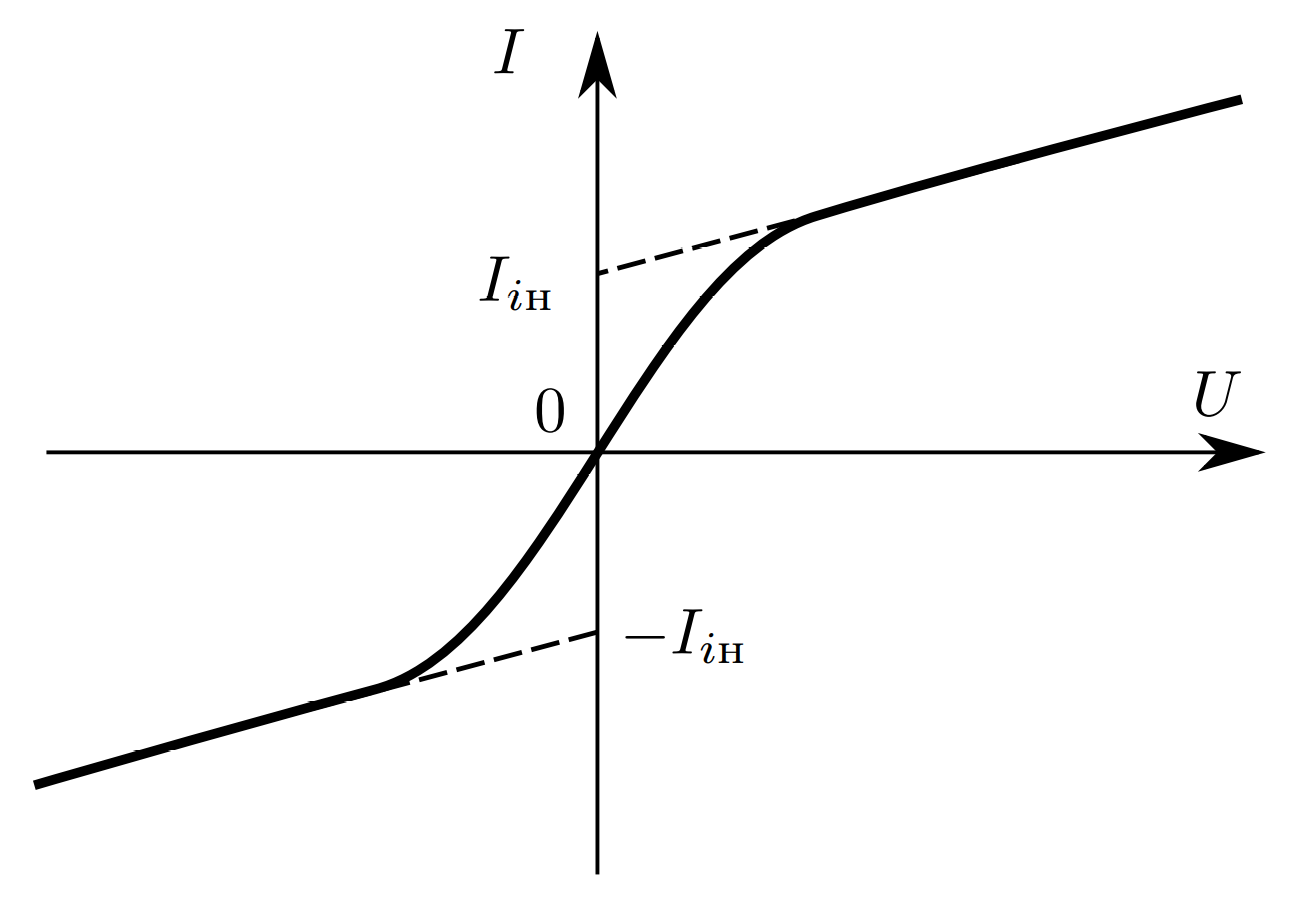
\includegraphics[width = 14 cm]{images/graph_cur.png}
        \caption{Вольт-амперная характеристика двойного зонда} 
        \label{theor_cur}
    \end{figure}

    Графики типа \ref{theor_cur} проще всего обрабатывать следующим образом. Сначала находится ток насыщения $I_{i\text{н}}$ из пересечения асимптот с осью $U = 0$. Затем находится наклон графика в начале координат, из которого можно определить температуру электронов $T_e$. Дифференциируя формулу для $I$ по $U$ в точке $U = 0$ и принимая во внимание, что при малых аргументах $\th{x}\approx x$, найдём \[k_{\text{Б}}T_e=\frac{1}{2}\frac{eI_{i\text{н}}}{\frac{\text{d}I}{\text{d}U}\vert{}_{U=0}},\] где $\frac{\text{d}I}{\text{d}U}\vert{}_{U=0}$ -- наклон характеристики зонда вблизи начала координат. По известным $T_e$ и $I_{i\text{н}}$ можно найти концентрацию заряженных частиц $n_i=n_e$.

    Таким образом, двойные зонды удобно применять для измерения электронной температуры и концентрации частиц в плазме.

    Вид ВАХ для конкретного газового проводника зависит от ряда условий, прежде всего от давления газа. На рис. \ref{graph:theor_VAC} представлен пример полученной экспериментально ВАХ разряда в неоне.
    
    В отсутствие внешнего ионизатора начальный участок характеристики несамостоятельного разряда (участок ОА) соответствует столь малым токам, что на графике его не удаётся изобразить. Участок АБ соответствует току насыщения и режиму \textit{газового усиления}. В точке В происходит пробой и начинается самостоятельный разряд. На участке ВГ уже выполнен критерий Таунсенда, но токи и степень ионизации ещё слишком малы, чтобы вызвать свечение и такой разряд называют \textit{тёмным таунсендовским}.
    
    \textit{Тлеющему разряду} соответствует участок ГДЕЖ. Участок \textit{ГД} называется \textit{поднормальным} тлеющим разрядом, почти вертикальная часть ДЕ -- \textit{нормальным} тлеющим разрядом и остальная часть ЕЖ -- \textit{аномальным} тлеющим разрядом.
    
    Нормальный тлеющий разряд обладает примечательным свойством самоорганизации: при увеличении полного тока в разряде, его плотность остаётся практически неизменной, меняется лишь площадь <<катодного пятна>>, из которого вытекает ток. Меняя $\mathcal{E}$ или $R$, можно видеть, как светящееся пятно на поверхности катода расширяется или сокращается. При этом напряжение в разряде практически не меняется. При полном заполнении катода дальнейшее увеличение тока будет возможно только за счёт повышения интенсивности ионизации газа, что возможно только при повышении напряжения. Разряд при этом переходит в режим аномального тлеющего разряда.
    
    Далее идёт спадающий участок ЖЗ, соответствующий разогреву катода и переходу к \textit{дуговому разряду}. Заметим, что при больших давлениях газа (атмосферном и больше) после пробоя сразу устанавливается дуговой разряд.
    
    \begin{figure}[H]
        \centering
        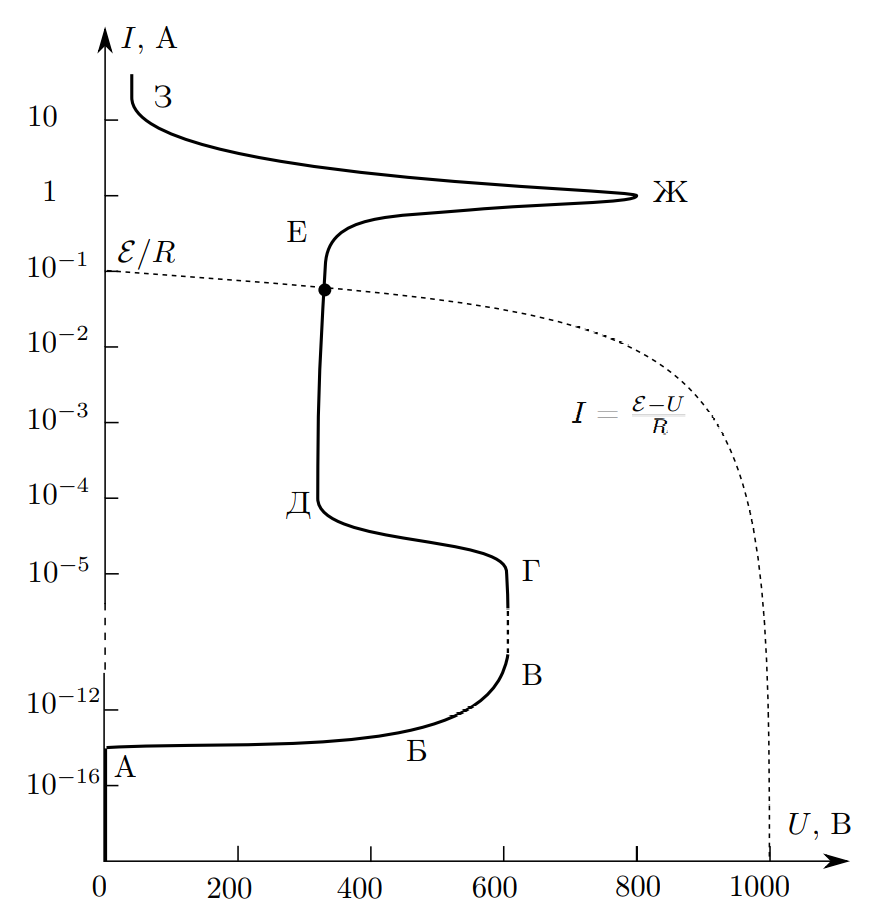
\includegraphics[width = 14 cm]{images/theor_graph_VAC.png}
        \caption{Вольт-амперная характеристика разряда в неоне} 
        \label{graph:theor_VAC}
    \end{figure}

    \newpage
    
    \section{Методика измерений и экспериментальная установка}

    Схема установки для исследования плазмы газового разряда в неоне представлена на рис. \ref{installation}. Стеклянная газоразрядная трубка имеет холодный (ненагреваемый) полый катод, три анода и \textit{геттерный узел} -- стеклянный баллон, на внутреннюю поверхность которого напылена газопоглощающая плёнка (\textit{геттер}). Трубка наполнена изотопом неона $^{22}\text{Ne}$ при давлении 2 мм рт. ст. Катод и один из анодов с помощью переключателя $\text{П}_1$ подключаются через балластный резистор $R_\text{б}$ ($\sim 450$ кОм) к регулируемому высоковольтному источнику питания (ВИП) с выходным напряжением до 5 кВ.

    \begin{figure}[H]
        \centering
        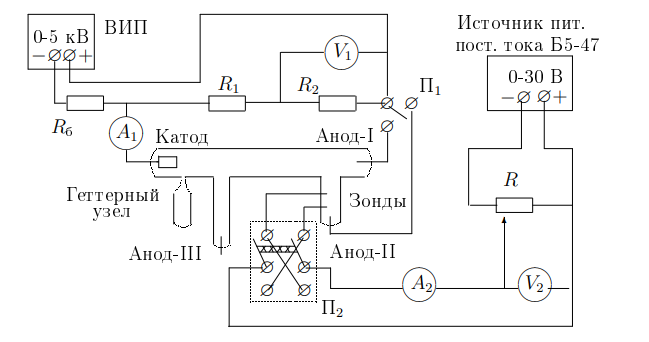
\includegraphics[width = 14 cm]{images/installation.png}
        \caption{Схема установки для исследования газового разряда}
        \label{installation}
    \end{figure}

    При подключении к ВИП анода-I между ним и катодом возникает газовый разряд. Ток разряда измеряется миллиамперметром $A_1$, а падение напряжения на разрядной трубке -- цифровым вольтметром $V_1$ (мультиметром GDM), подключённым к трубке через высокоомный (25 МОм) делитель напряжения с коэффициентом $\left( R_1 + R_2 \right)/R_2 = 10$.
    
    При подключении к ВИП анода-II разряд возникает в пространстве между катодом и анодом-II, где находится двойной зонд, используемый для диагностики плазмы положительного столба. Зонды изготовлены из молибденовой проволоки диаметром $d = 0,2$ мм и имеют длину $l = 5,2$ мм. Они подключены к источнику питания GPS через потенциометр $R$. Переключатель $\text{П}_2$ позволяет изменять полярность напряжения на зондах. Величина напряжения на зондах изменяется с помощью дискретного переключателя <<V>> выходного напряжения источника питания и потенциометра $R$, а измеряется цифровым вольтметром $V_2$ (GDM). Для измерения зондового тока используется мультиметр $А_2$ (GDM). Анод-III в нашей работе не используется.

    \newpage
	
    \section{Результаты измерений и обработка данных}

    \subsection{Вольт-амперная характеристика разряда}

     Определим напряжение зажигания разряда. Для этого будем плавно поднимать напряжение ВИП. В момент зажигания разряда $U_\text{заж} = 1960$ В. Проведем измерения ВАХ газоразрядной трубки с помощью амперметра $A_1$ и вольтметра $V_1$. Результаты измерений приведены в таблице \ref{table:VAC}.

     \begin{table}[H]
        \centering
        \begin{tabular}{|c|c|}
        \hline
        $I_p,$ мА & $U_p$, В \\ \hline
        0,505 & 34,26 \\ \hline
        0,946 & 32,43 \\ \hline
        1,582 & 31,26 \\ \hline
        1,998 & 30,29 \\ \hline
        2,526 & 27,39 \\ \hline
        2,524 & 27,40 \\ \hline
        3,052 & 25,17 \\ \hline
        3,589 & 23,47 \\ \hline
        4,093 & 23,18 \\ \hline
        4,495 & 22,90 \\ \hline
        5,051 & 22,35 \\ \hline
        4,029 & 22,87 \\ \hline
        3,036 & 25,25 \\ \hline
        2,049 & 29,81 \\ \hline
        1,077 & 32,14 \\ \hline
        0,548 & 34,05 \\ \hline
        \end{tabular}
        \caption{Зависимость напряжения разряда $U_p$ от его тока $I_p$}
        \label{table:VAC}
    \end{table}
             
     По данным таблицы \ref{table:VAC} построим график зависимости $U_p(I_p)$ (рис. \ref{graph:VAC}). 
     
     \begin{figure}[H]
         \centering
         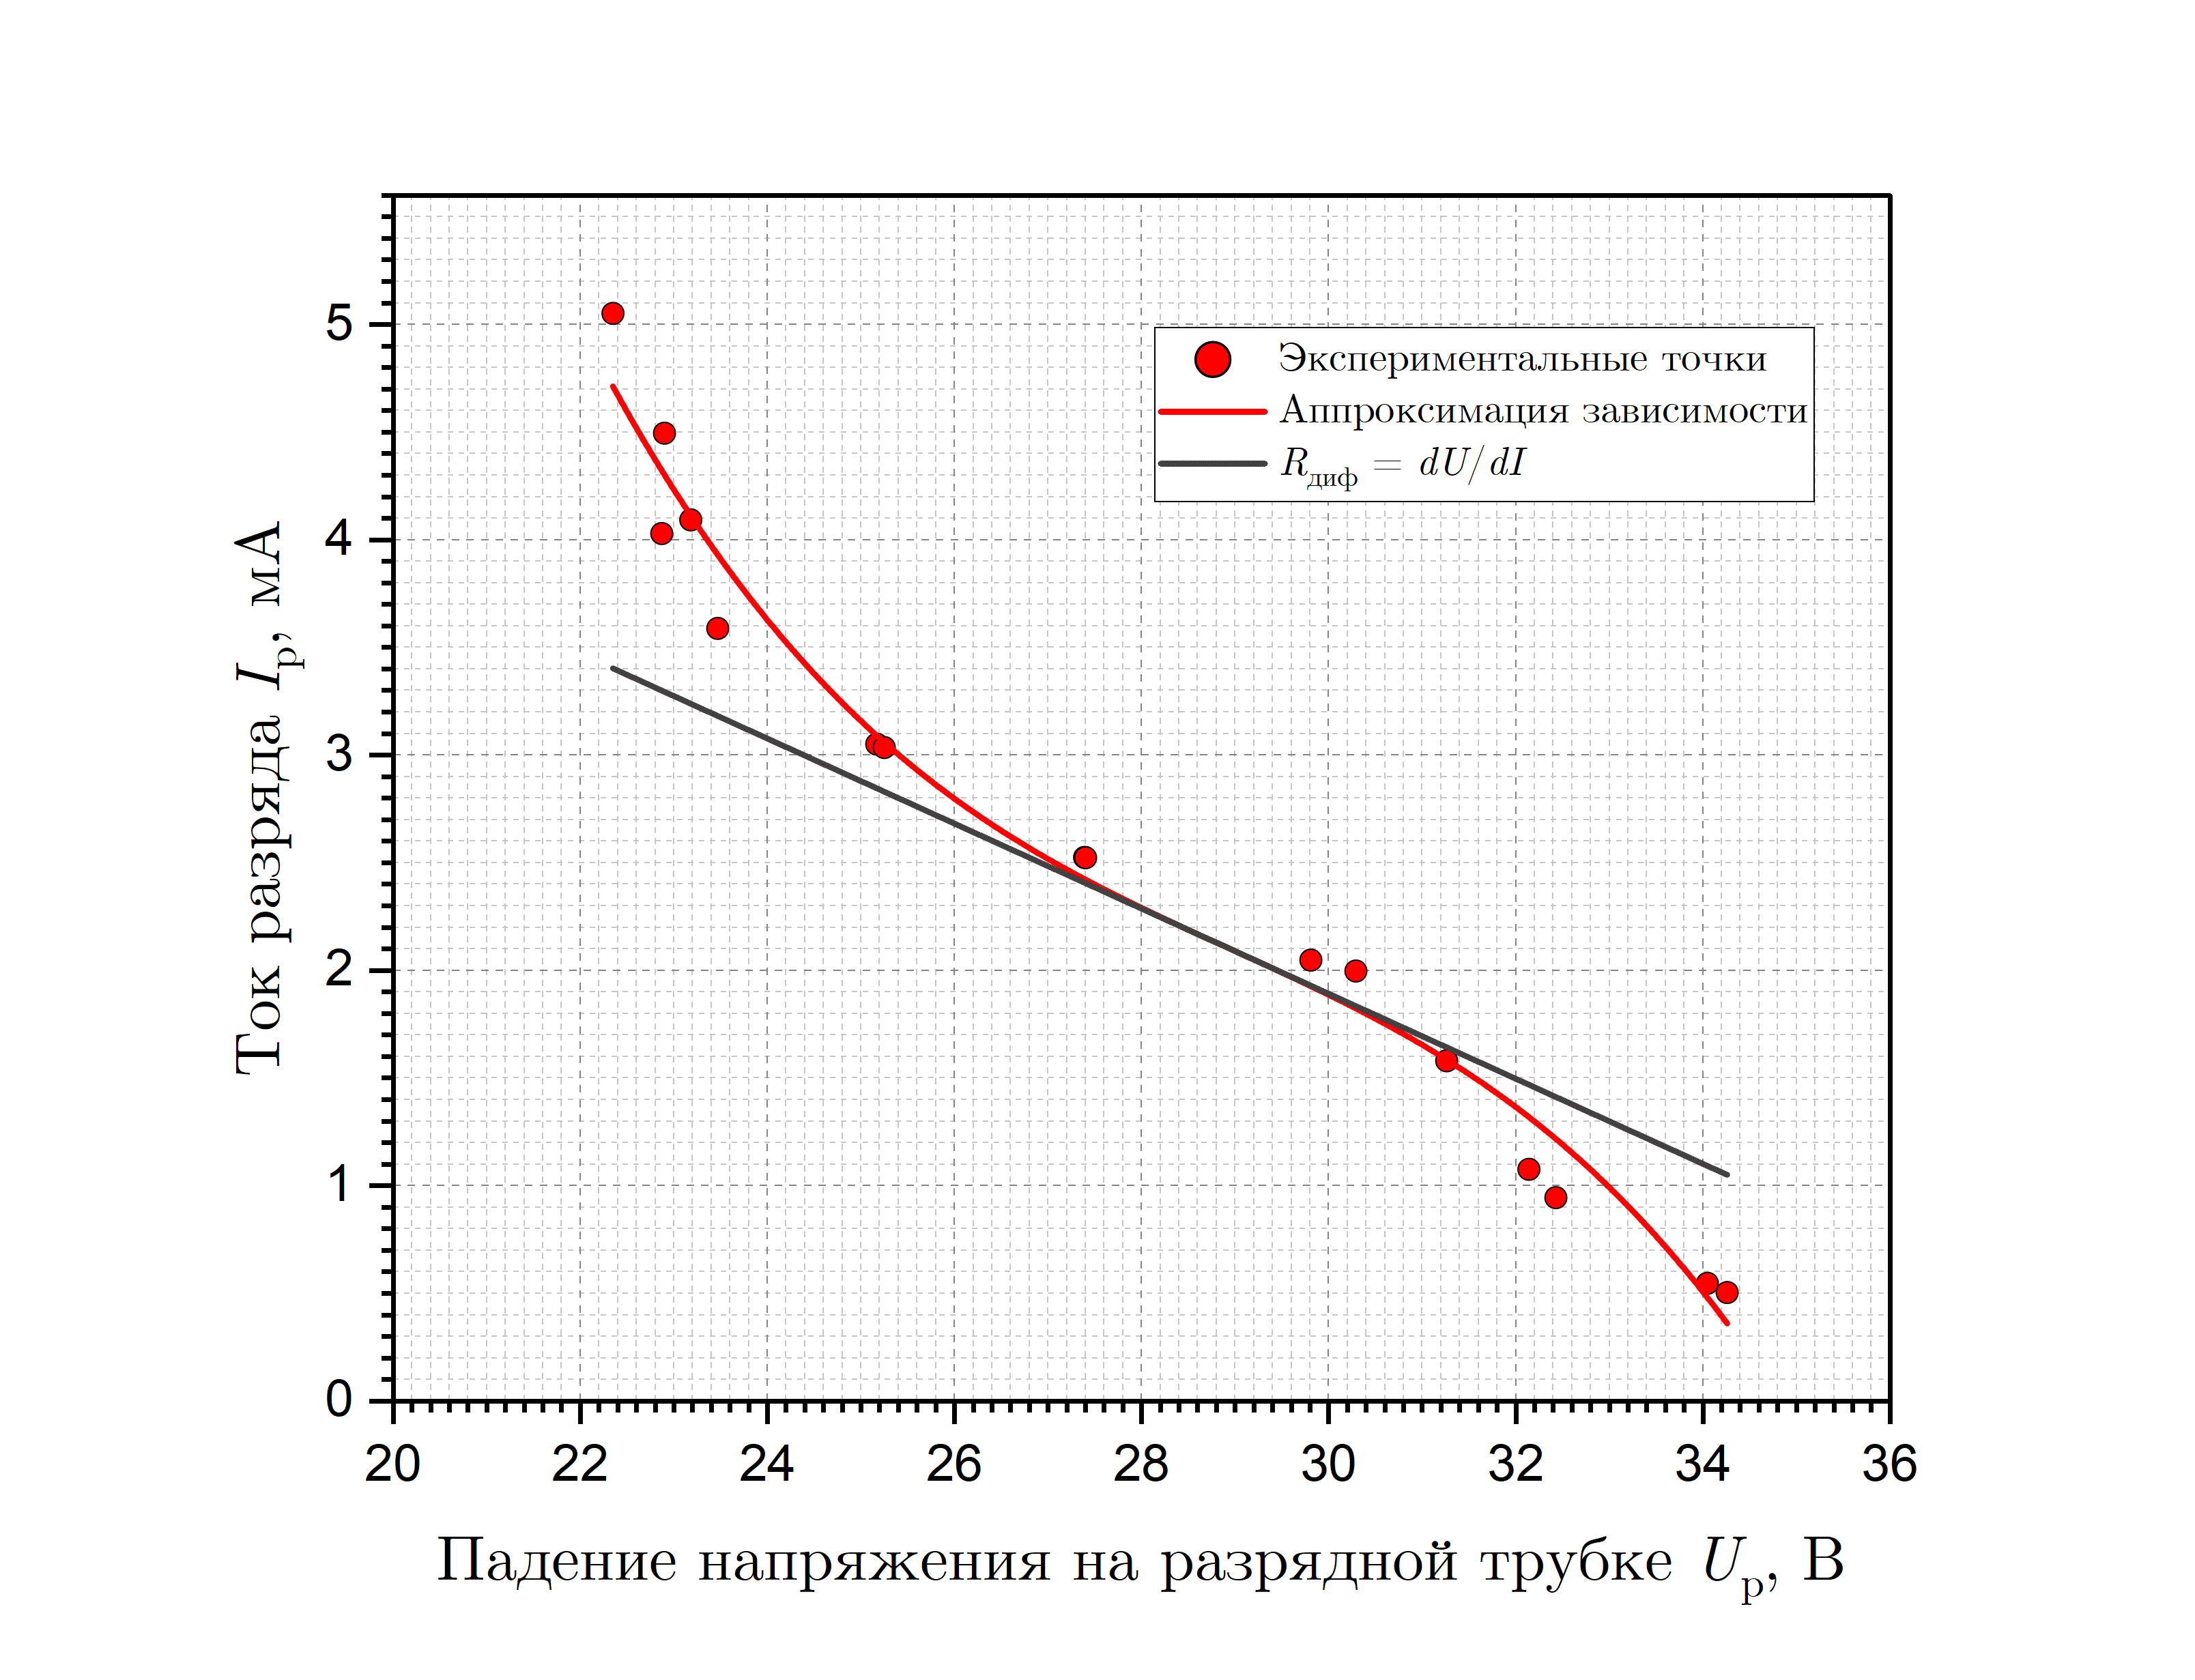
\includegraphics[width = 14 cm]{images/graph_VAC.png}
         \caption{Вольт-амперная характеристика разряда в координатах $I_p(U_p)$}
         \label{graph:VAC}
     \end{figure}
     
     Сравнив график с рисунком \ref{graph:theor_VAC}, сделаем вывод, что полученный в работе график соответствует участку \textit{Г-Д} (\textit{поднормальный тлеющий разряд}). С помощью программы \textit{Origin Pro 2023b} также определим максимальное дифференциальное сопротивление разряда $R_\text{дифф}$:

     \begin{equation}
         R_\text{дифф} = \frac{dU}{dI} = -5,06 \text{ кОм}.
     \end{equation}

    \subsection{Зондовые характеристики}

    Подготовим приборы к работе, затем плавно увеличим напряжение ВИП до возникновения разряда. Установим максимально допустимое значение разрядного тока $I_{\text{р}}^{max} = 5,0 ~ \text{мА}$. Подготовим к работе источник питания, после чего с помощью потенциометра $R$ установим на зонде максимально допустимое напряжение $U_{\text{з}}^{max} = 25,0~\text{В}$.
        
    Измерим вольт-амперную характеристику двойного зонда $I_{\text{з}} \left( U_{\text{з}} \right)$ в диапазоне от $-U^{max}_{\text{з}}$ до $U^{max}_{\text{з}}$ при фиксированном токе разряда $I_{\text{р}}$. Проведём данные измерения при трёх различных значениях тока разряда. Занесём полученные данные в таблицу \ref{table:probes}.

    \begin{table}[H]
        \centering
        \begin{tabular}{|cc|cc|cc|}
        \hline
        \multicolumn{2}{|c|}{$I_p = 5,05 \text{ мА}$} & \multicolumn{2}{c|}{$I_p = 3,02 \text{ мА}$} & \multicolumn{2}{c|}{$I_p = 1,51 \text{ мА}$} \\ \hline
        \multicolumn{1}{|c|}{$I_\text{з}$, мкА} & $U_\text{з}$ , В & \multicolumn{1}{c|}{$I_\text{з}$} & $U_\text{з}$ , В & \multicolumn{1}{c|}{$I_\text{з}$} & $U_\text{з}$ , В \\ \hline
        \multicolumn{1}{|c|}{117,12} & 25,01 & \multicolumn{1}{c|}{69,30} & 25,00 & \multicolumn{1}{c|}{36,01} & 25,05 \\ \hline
        \multicolumn{1}{|c|}{114,30} & 22,04 & \multicolumn{1}{c|}{67,24} & 22,02 & \multicolumn{1}{c|}{34,75} & 22,04 \\ \hline
        \multicolumn{1}{|c|}{111,32} & 19,03 & \multicolumn{1}{c|}{65,20} & 19,03 & \multicolumn{1}{c|}{33,50} & 19,01 \\ \hline
        \multicolumn{1}{|c|}{107,70} & 16,20 & \multicolumn{1}{c|}{63,10} & 16,04 & \multicolumn{1}{c|}{32,30} & 16,12 \\ \hline
        \multicolumn{1}{|c|}{101,60} & 13,15 & \multicolumn{1}{c|}{60,33} & 13,10 & \multicolumn{1}{c|}{30,87} & 13,03 \\ \hline
        \multicolumn{1}{|c|}{92,02} & 10,10 & \multicolumn{1}{c|}{55,80} & 10,13 & \multicolumn{1}{c|}{28,80} & 10,13 \\ \hline
        \multicolumn{1}{|c|}{83,20} & 8,09 & \multicolumn{1}{c|}{50,95} & 8,12 & \multicolumn{1}{c|}{26,60} & 8,05 \\ \hline
        \multicolumn{1}{|c|}{72,30} & 6,10 & \multicolumn{1}{c|}{44,10} & 6,08 & \multicolumn{1}{c|}{23,55} & 6,14 \\ \hline
        \multicolumn{1}{|c|}{58,80} & 4,01 & \multicolumn{1}{c|}{35,20} & 4,04 & \multicolumn{1}{c|}{18,99} & 3,05 \\ \hline
        \multicolumn{1}{|c|}{45,50} & 2,10 & \multicolumn{1}{c|}{24,50} & 2,05 & \multicolumn{1}{c|}{13,08} & 2,02 \\ \hline
        \multicolumn{1}{|c|}{33,33} & 0,55 & \multicolumn{1}{c|}{15,00} & 0,50 & \multicolumn{1}{c|}{8,20} & 0,56 \\ \hline
        \multicolumn{1}{|c|}{-11,60} & -0,56 & \multicolumn{1}{c|}{-3,20} & -0,55 & \multicolumn{1}{c|}{3,92} & -0,48 \\ \hline
        \multicolumn{1}{|c|}{-23,40} & -2,02 & \multicolumn{1}{c|}{-6,02} & -2,03 & \multicolumn{1}{c|}{-1,84} & -2,10 \\ \hline
        \multicolumn{1}{|c|}{-38,67} & -4,04 & \multicolumn{1}{c|}{-17,50} & -4,04 & \multicolumn{1}{c|}{-7,75} & -4,04 \\ \hline
        \multicolumn{1}{|c|}{-52,37} & -6,03 & \multicolumn{1}{c|}{-27,20} & -6,07 & \multicolumn{1}{c|}{-12,90} & -6,08 \\ \hline
        \multicolumn{1}{|c|}{-64,47} & -8,02 & \multicolumn{1}{c|}{-34,70} & -8,13 & \multicolumn{1}{c|}{-16,62} & -8,11 \\ \hline
        \multicolumn{1}{|c|}{-74,70} & -10,14 & \multicolumn{1}{c|}{-39,90} & -10,04 & \multicolumn{1}{c|}{-19,10} & -10,01 \\ \hline
        \multicolumn{1}{|c|}{-84,87} & -13,10 & \multicolumn{1}{c|}{-44,50} & -13,00 & \multicolumn{1}{c|}{-21,32} & -13,07 \\ \hline
        \multicolumn{1}{|c|}{-90,93} & -16,03 & \multicolumn{1}{c|}{-47,80} & -16,04 & \multicolumn{1}{c|}{-22,35} & -16,05 \\ \hline
        \multicolumn{1}{|c|}{-94,70} & -19,05 & \multicolumn{1}{c|}{-49,65} & -19,06 & \multicolumn{1}{c|}{-23,13} & -19,01 \\ \hline
        \multicolumn{1}{|c|}{-97,70} & -22,06 & \multicolumn{1}{c|}{-51,40} & -22,10 & \multicolumn{1}{c|}{-23,93} & -22,02 \\ \hline
        \multicolumn{1}{|c|}{-100,66} & -25,05 & \multicolumn{1}{c|}{-53,20} & -25,05 & \multicolumn{1}{c|}{-24,74} & -25,05 \\ \hline
        \end{tabular}
        \caption{Результаты измерения зависимости напряжения на зонде $U_\text{з}$ от тока $I_\text{з}$ через него}
        \label{table:probes}
    \end{table}

    Параметры используемого в работе зонда: $d = 0,2~\text{мм}$ и $l = 5,2~\text{мм}$.

    Построим теперь в отдельных системах координат отцентрированные зондовые характеристики для разных токов. Полученные зависимости приведены на рисунках \ref{graph:probes_5}, \ref{graph:probes_3} и \ref{graph:probes_1_5}.

    \begin{figure}[H]
        \centering
        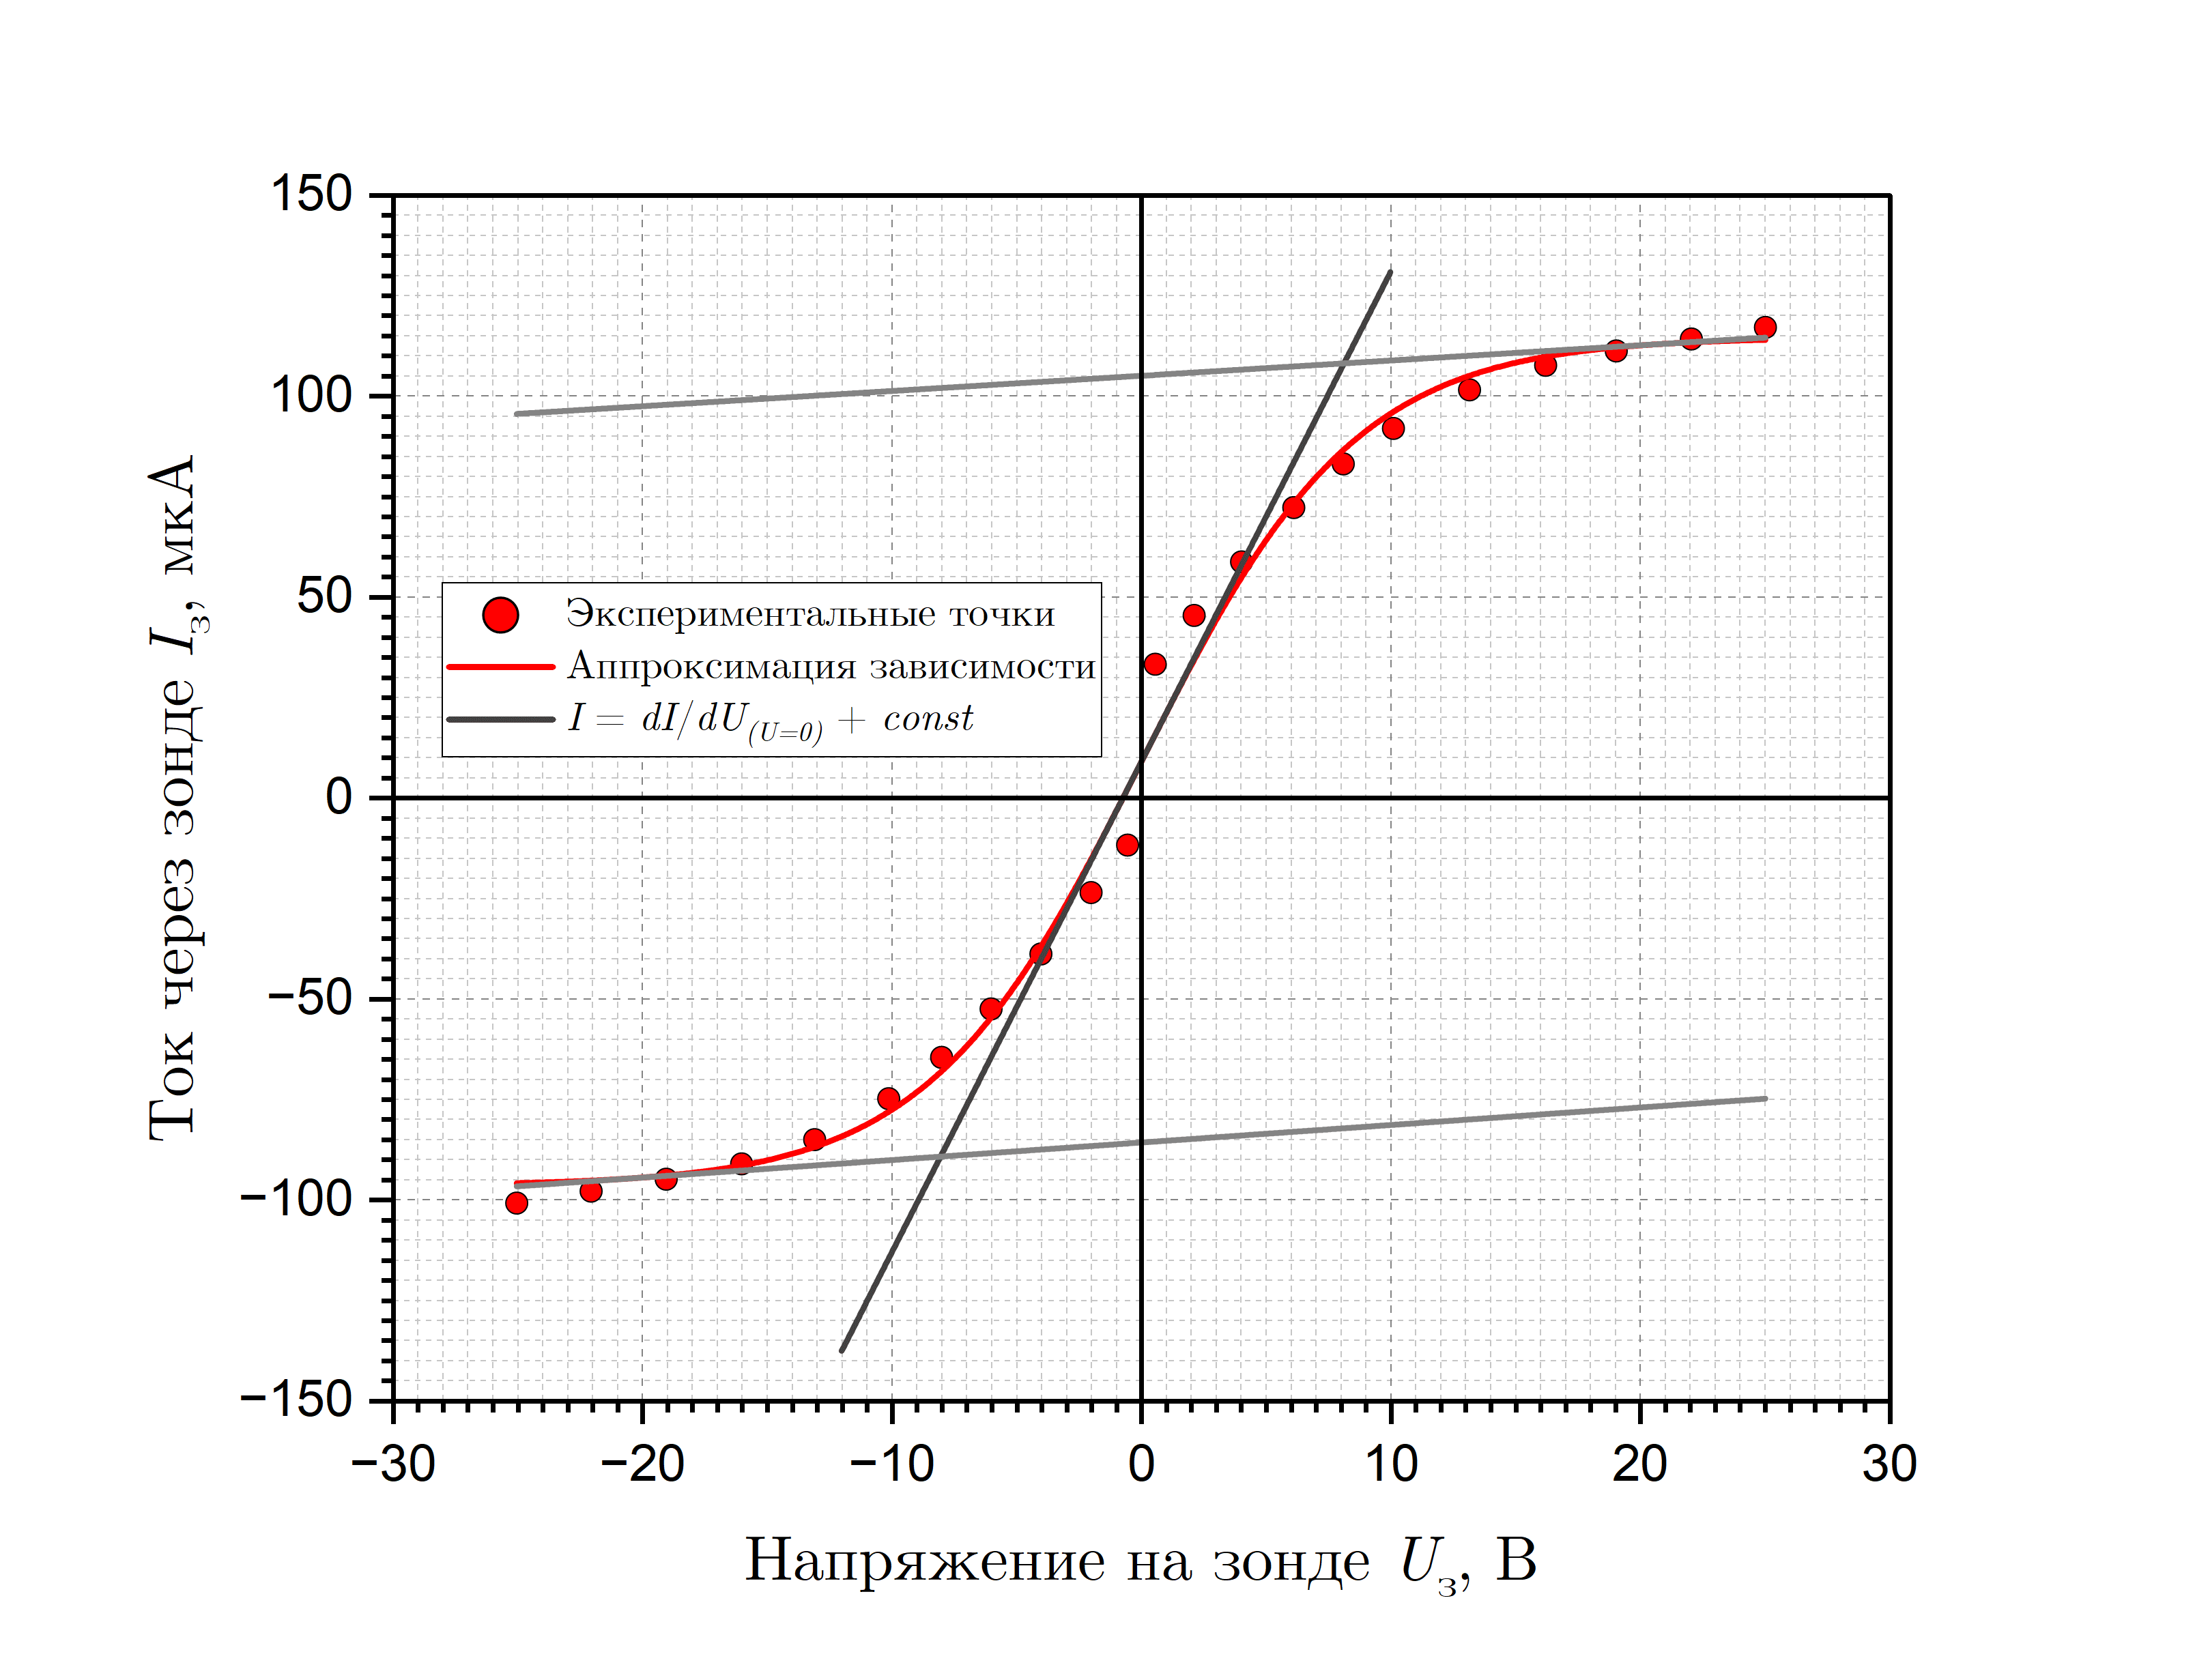
\includegraphics[width = 14 cm]{images/graph_5mA.png}
        \caption{Зондовая характеристика $I_{\text{з}}\left(U_{\text{з}}\right)$ при токе через разряд $I_{\text{р}}= 5 ~\text{мА}$}
            \label{graph:probes_5}
    \end{figure}

    \begin{figure}[H]
        \centering
        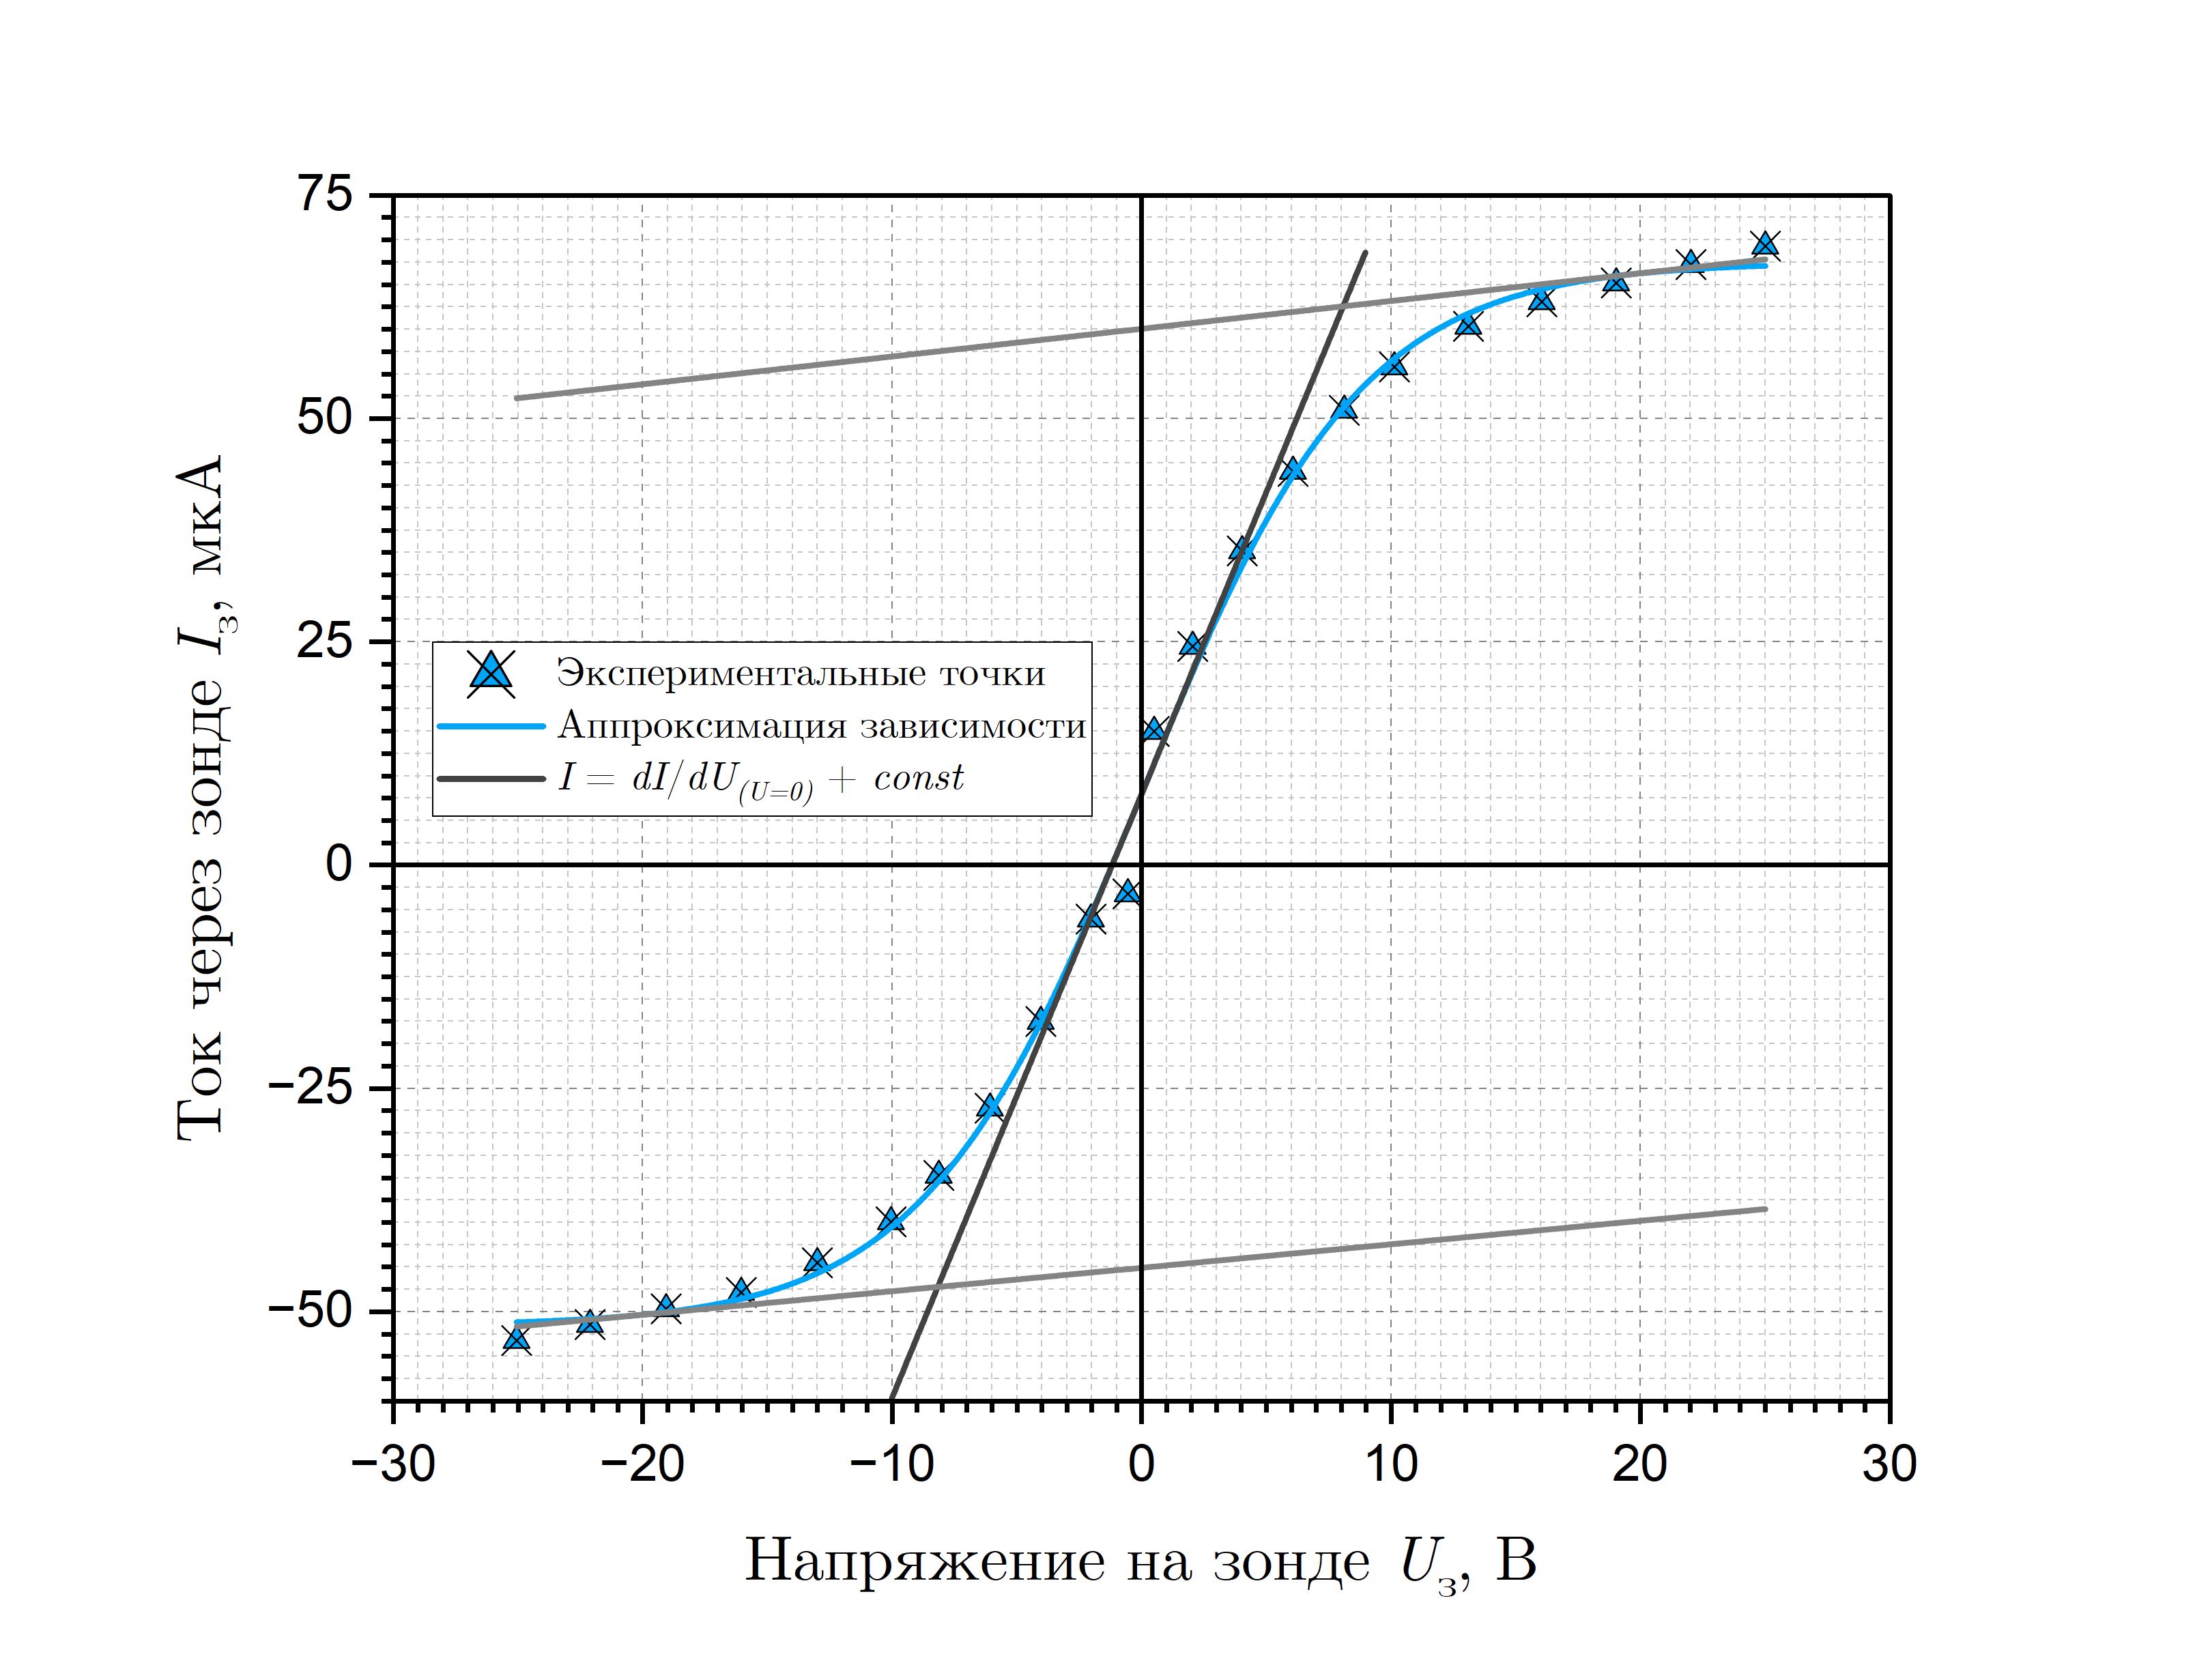
\includegraphics[width = 14 cm]{images/graph_3mA.png}
        \caption{Зондовая характеристика $I_{\text{з}}\left(U_{\text{з}}\right)$ при токе через разряд $I_{\text{р}}=3,0~\text{мА}$}
            \label{graph:probes_3}
    \end{figure}

    \begin{figure}[H]
        \centering
        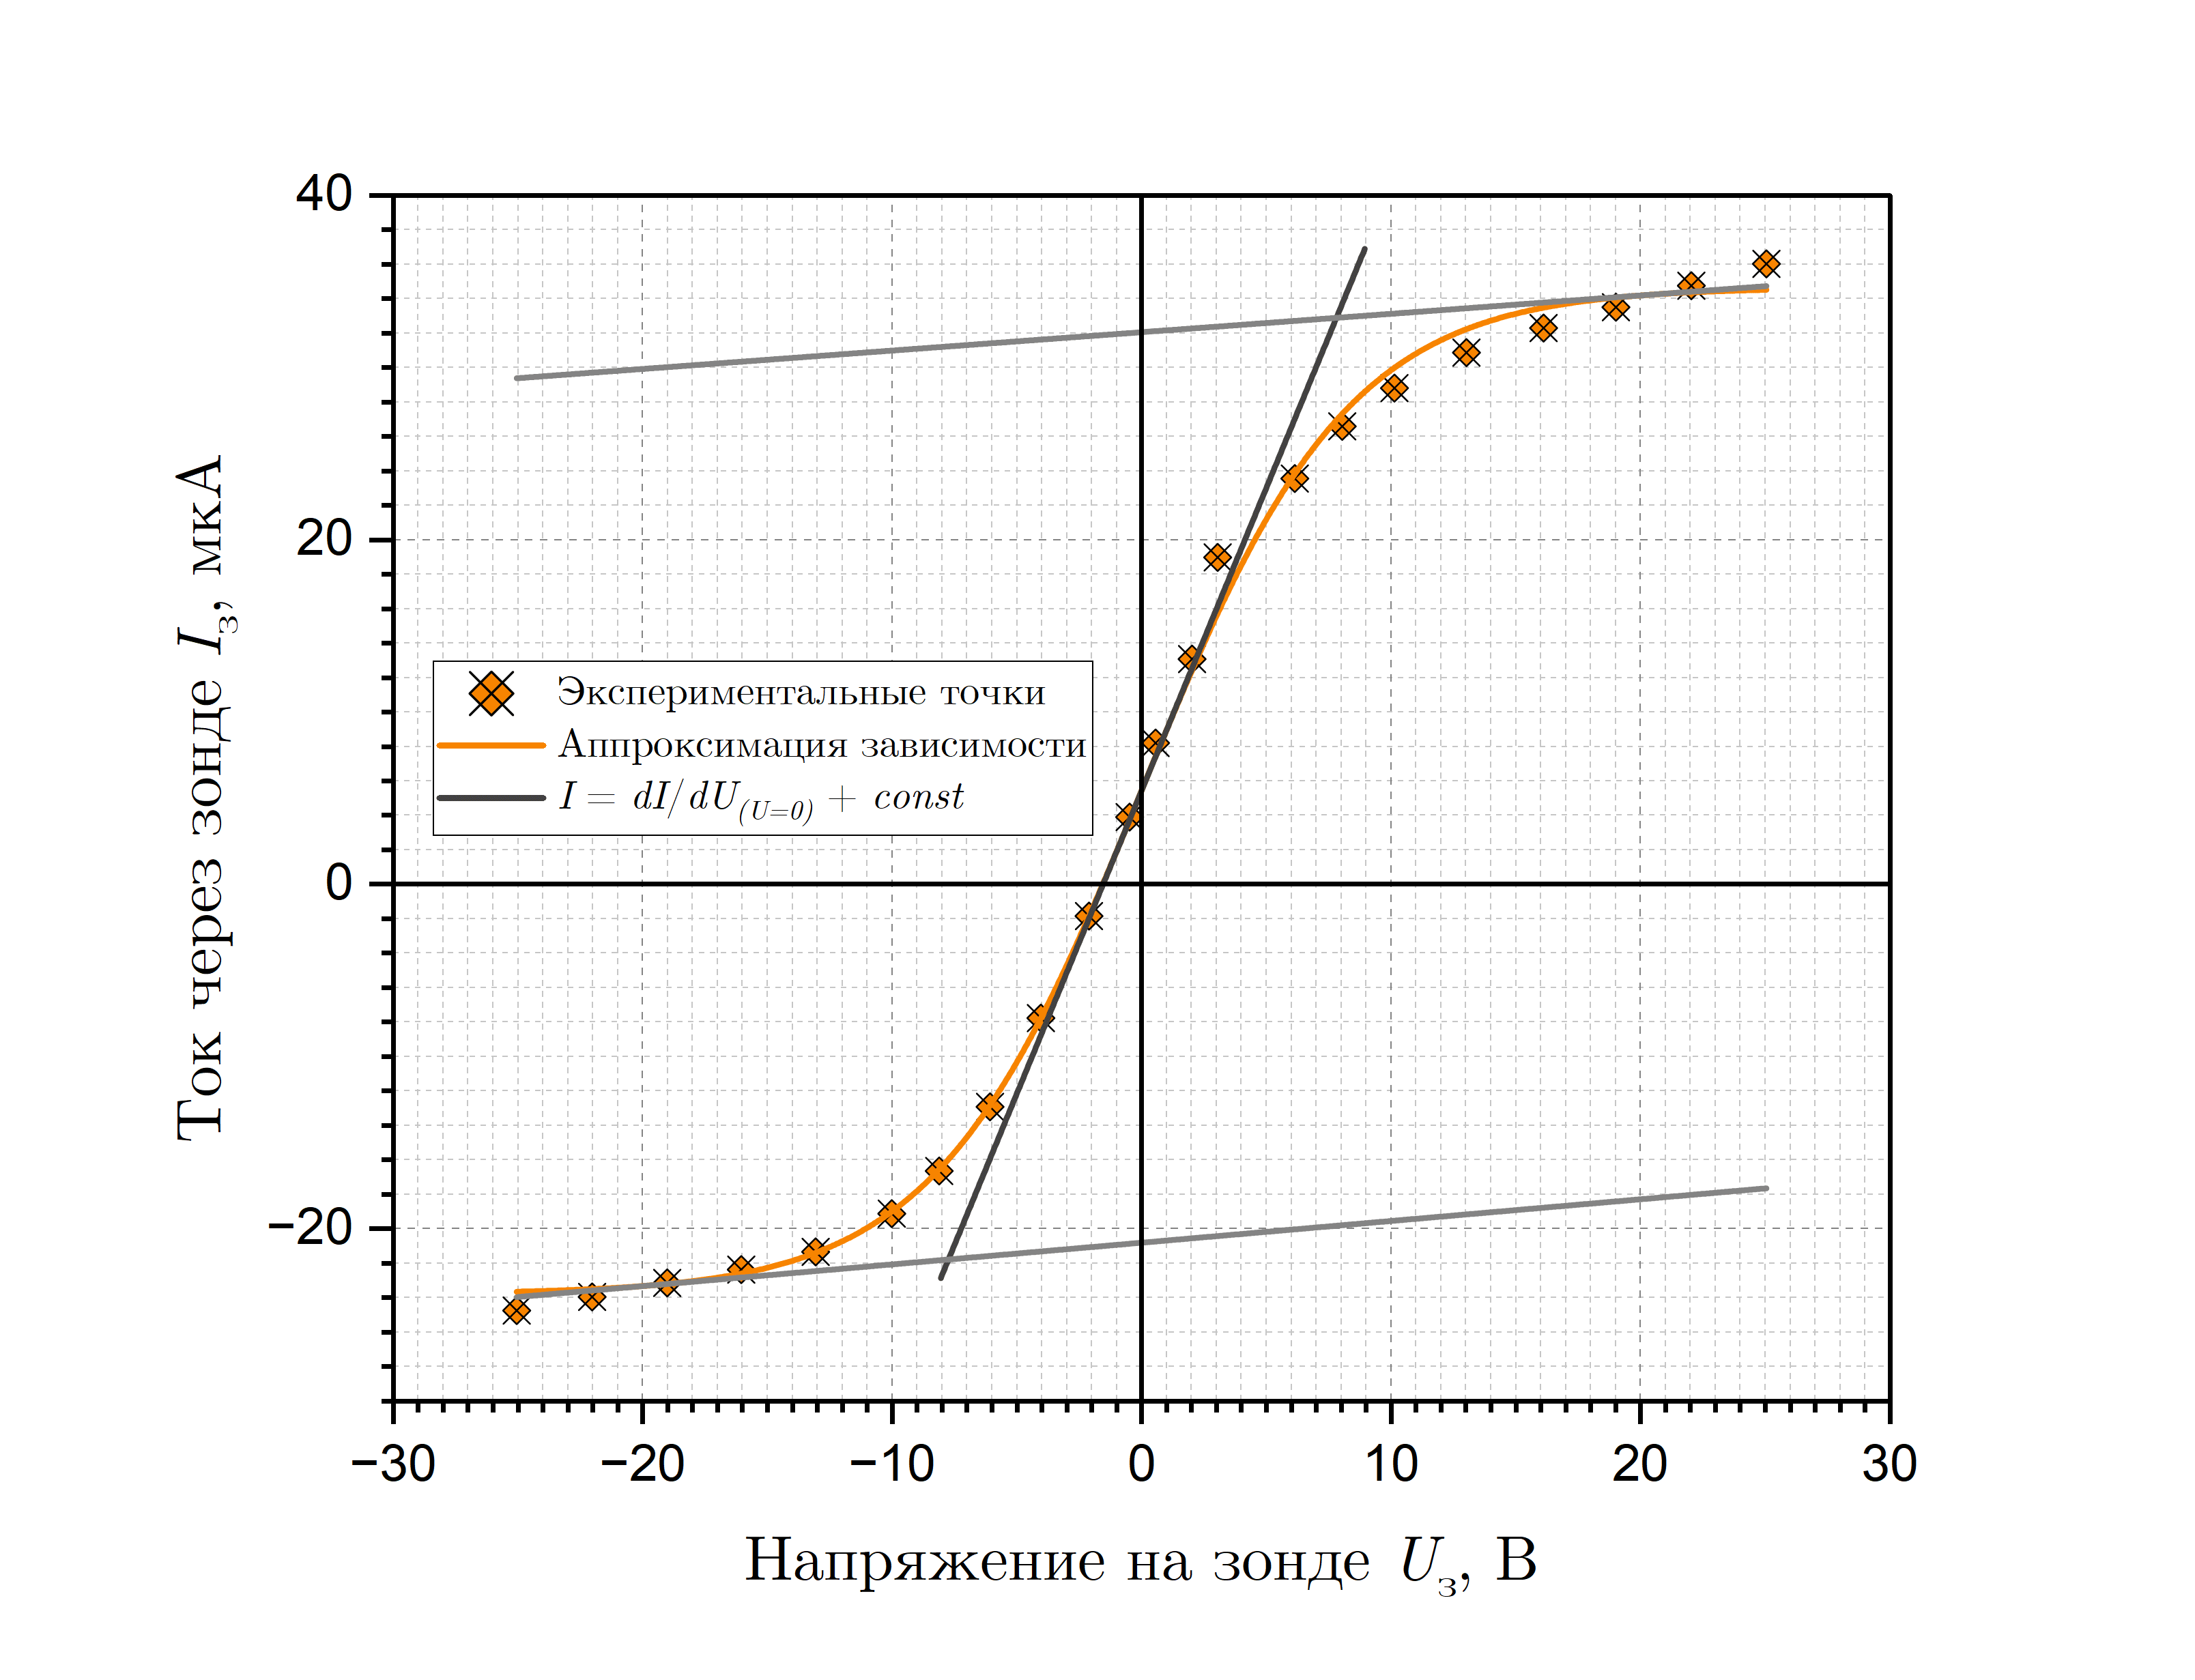
\includegraphics[width = 14 cm]{images/graph_1_5mA.png}
        \caption{Зондовая характеристика $I_{\text{з}}\left(U_{\text{з}}\right)$ при токе через разряд $I_{\text{р}}= 1,5 ~\text{мА}$}
            \label{graph:probes_1_5}
    \end{figure}
 
    По графикам определим температуру электронов. Проведём асимптоты к току насыщения до пересечения с осью $U = 0$, определив ток насыщения $I_{i\text{н}}$. После этого проведём касательную к зондовой характеристике в начале координат, определив $\frac{dI}{dU} \vert_{U = 0}$. Проведём горизонтали $I = I_{i\text{н}}$ до пересечения с касательной и определим значение $\Delta U$, затем $kT_e = \frac{e \Delta U}{2}$. Полученные из графиков значения $\Delta U^{\pm}$ и $T_e$ занесём в таблицу \ref{table:result_9}. Основным источников погрешности $T_e$ является неидеальность совпадения $\Delta U^{\pm}$ при разных полярностях напряжения на зонде, а также погрешности вольтметра и амперметра.

    \begin{table}[H]
	\centering
	\begin{tabular}{|c|c|c|c|}
		\hline
		$I_{\text{р}}$, мА & $5,05$ & $3,02$ & $1,51$ \\ \hline
		$I_{i\text{н}}^+$, мкА & 105,1 & 60,1 & 32,1 \\ \hline
		$I_{i\text{н}}^-$, мкА & 85,6 & 45,1 & 20,8 \\ \hline
		$\bar{I}_{i\text{н}}$, мкА & 95,4 & 52,6 & 26,5 \\ \hline
		$\Delta U^+$, В & 7,9 & 7,8 & 7,6 \\ \hline
		$\Delta U^-$, В & 7,7 & 7,8 & 7,5 \\ \hline
		$\Delta\bar{U}$, В & 7,8 & 7,8 & 7,6 \\ \hline
		$T_e,\ 10^4~\text{К}$ & 4,6 & 4,6 & 4,5 \\ \hline
	\end{tabular}
        \caption{Зависимость температуры электронов $T_e$ от тока $I_{\text{р}}$ через разряд} 
        \label{table:result_9}
    \end{table}

    Построим на одном листе семейство зондовых характеристик (рис. \ref{graph:probes}).

    \begin{figure}[H]
        \centering
        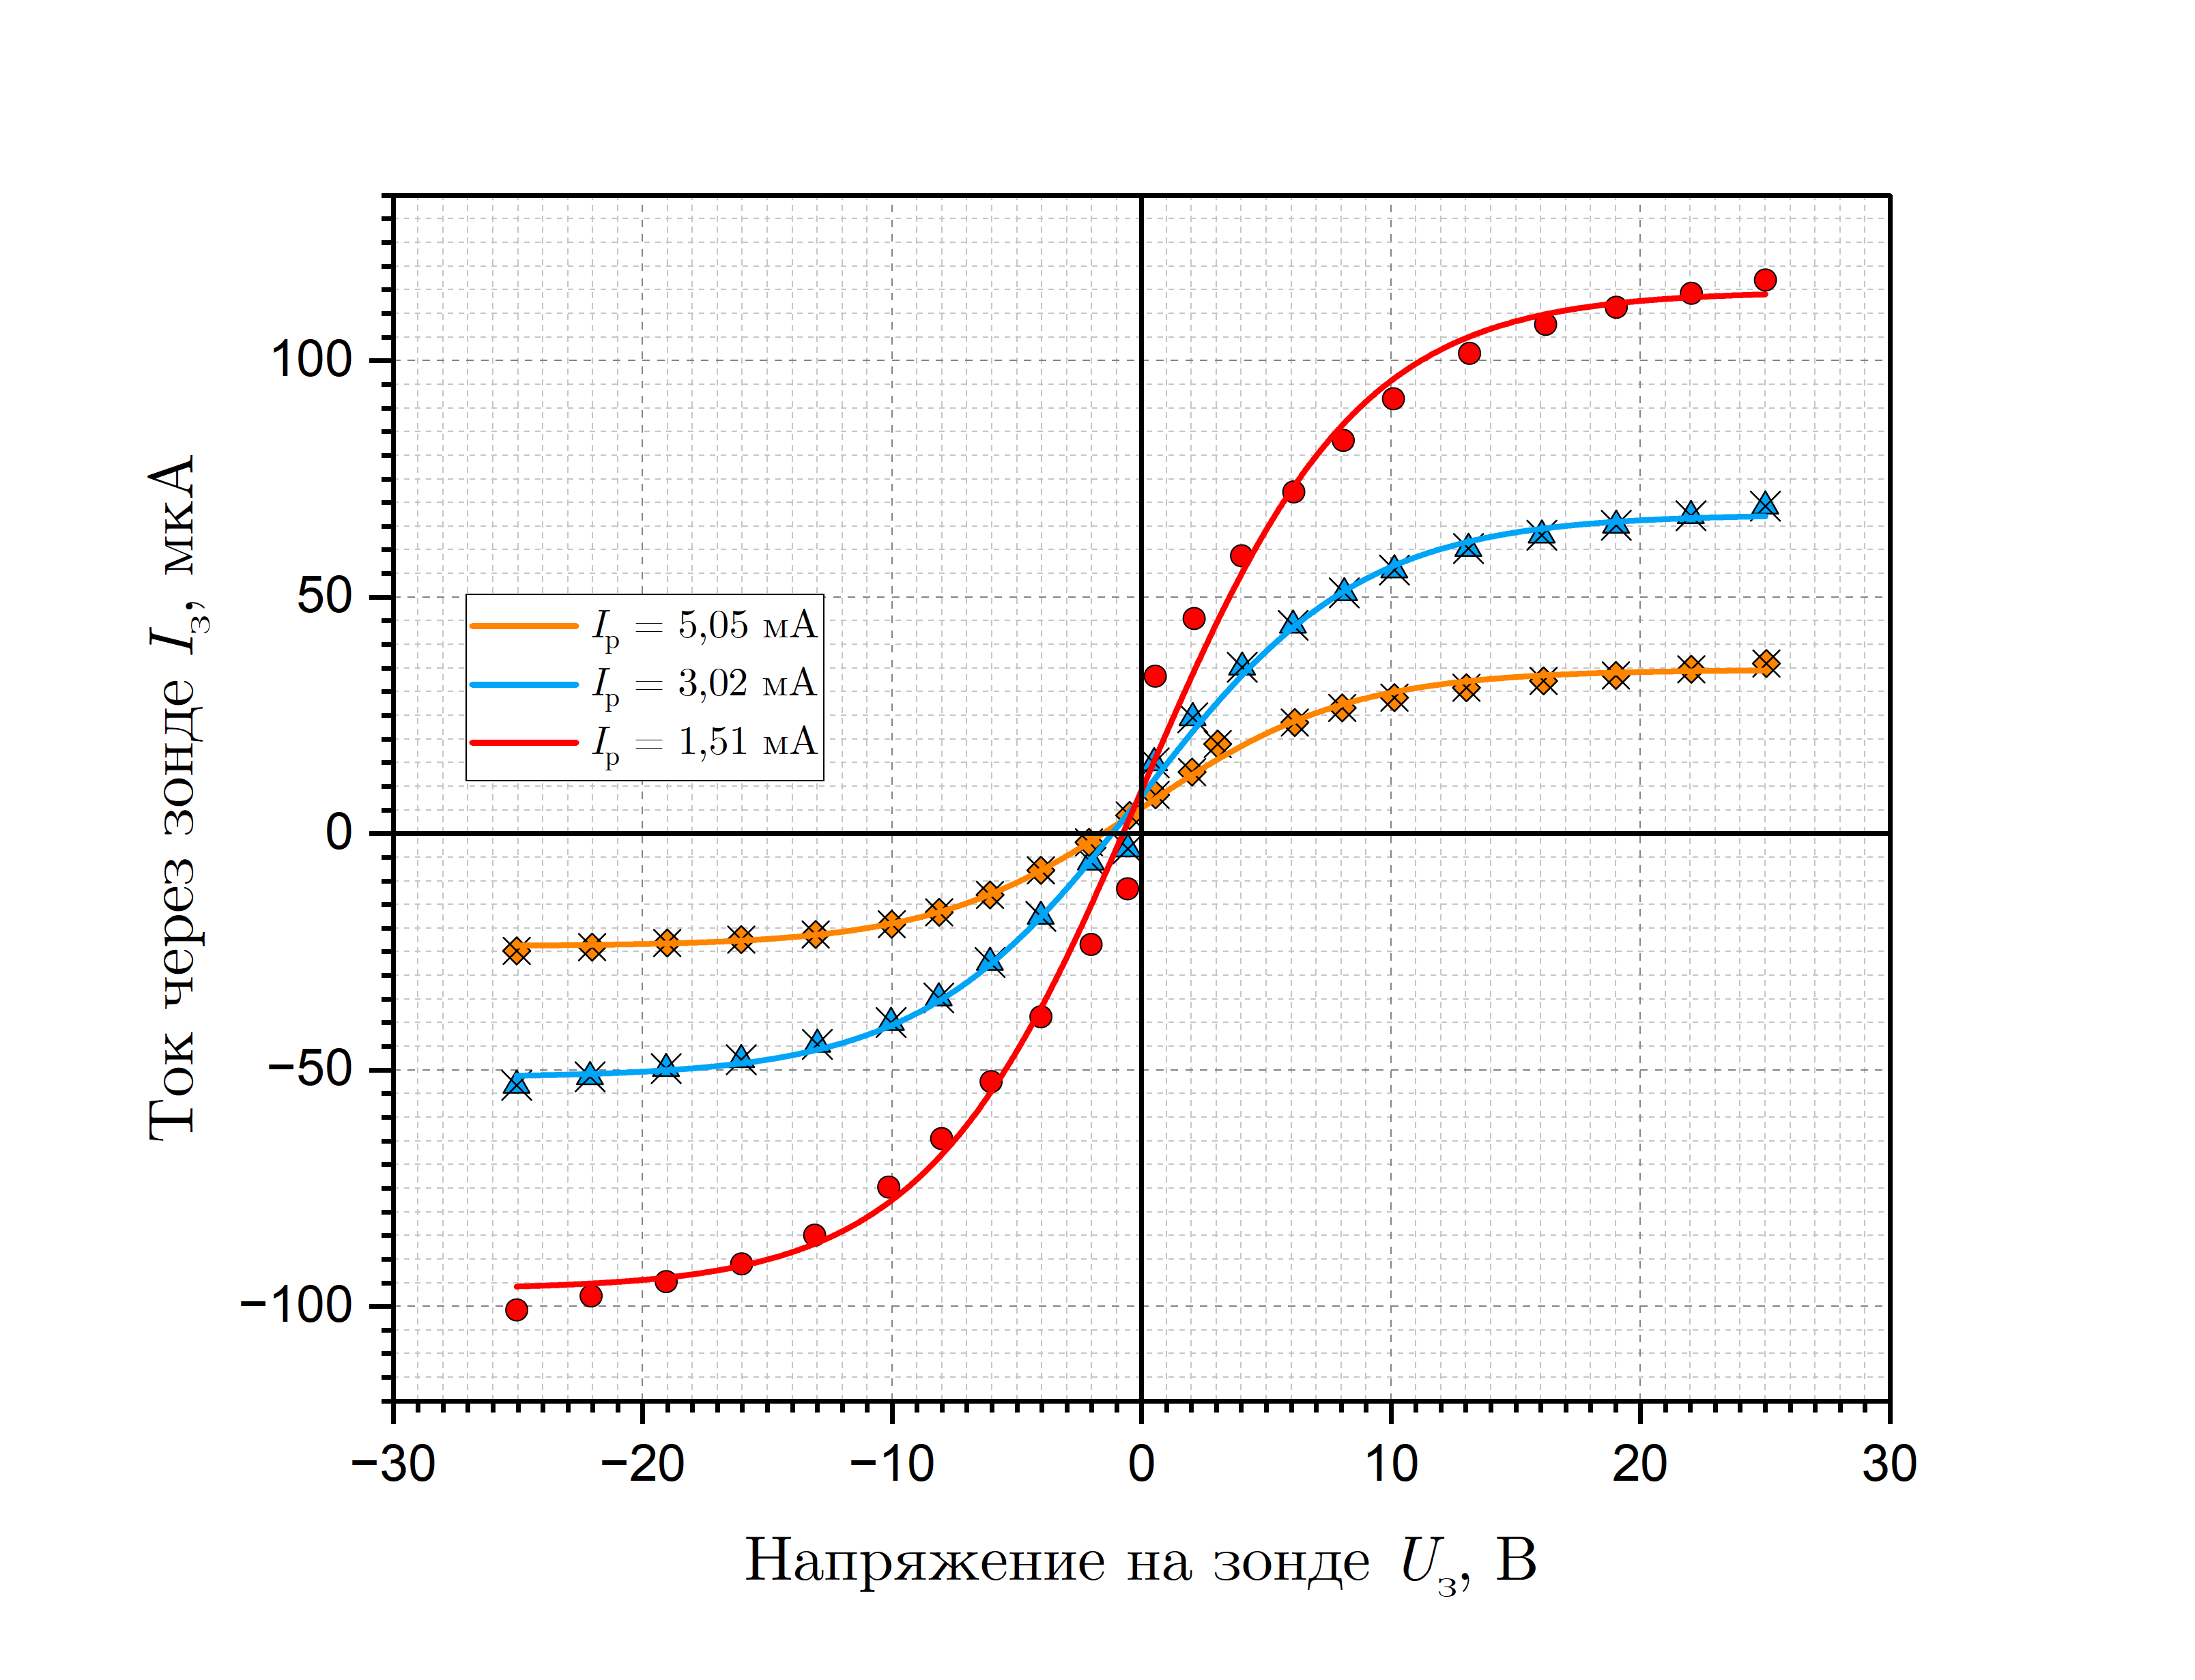
\includegraphics[width = 14 cm]{images/graph_probes.png}
        \caption{Семейство зондовых характеристик $I_{\text{з}}\left(U_{\text{з}}\right)$} 
        \label{graph:probes}
    \end{figure}
    
    Определим концентрацию электронов $n_e$, считая её равной концентрации ионов $n_i$ и используя \textit{формулу Бома}:
    \begin{equation}
        I_{i\text{н}} = 0,4n_e eS \sqrt{\frac{2kT_e}{m_i}} \implies n_e = \frac{2,5I_{i\text{н}}}{eS} \sqrt{\frac{m_i}{2kT_e}} = \frac{2,5I_{i\text{н}}}{\pi dle}\sqrt{\frac{m_i}{\Delta U}},
    \end{equation}
    
    где $S=\pi dl$ -- площадь поверхности зонда, а $m_i=22\cdot1,66\cdot10^{-27}~\text{кг}$ -- масса иона неона. Посчитанные по формуле значения $n_e$ тоже занесём в таблицу \ref{table:results}.

    Зная концентрацию электронов в плазме, можно найти их плазменную частоту колебаний по формуле

    \begin{equation}
        \omega_p = \sqrt{\frac{4\pi n_ee^2}{m_e}}\ \left[\text{СГС}\right] = 5,6 \cdot 10^4 \sqrt{n_e}\ \left[\text{СГС}\right] = 5,6 \sqrt{n_e}\ \left[\text{СИ}\right].
    \end{equation}
    
    Результаты также занесём в таблицу \ref{table:results}. Заметим, что при падении на эту плазму электромагнитного излучения через неё пройдут волны с частотами, \textit{превышающими} $\omega_p$.

    Рассчитаем теперь электронную поляризационную длину $r_{D_e}$. Используем формулу

    \begin{equation}
        r_{D_e} = \sqrt{\frac{kT_e}{4\pi n_ee^2}} = \frac{1}{\omega_p} \sqrt{\frac{e\Delta U}{2m_e}}.
    \end{equation}
    
    Занесём результаты в таблицу \ref{table:results}.

    Найдём \textit{дебаевский радиус}, учитывая $T_i\approx300~\text{К}$, по формуле

    \begin{equation}
        r_{D} = \sqrt{\frac{kT_i}{4\pi n_ee^2}} = \frac{1}{\omega_p} \sqrt{\frac{kT_i}{m_e}}.
    \end{equation}
    
     Занесём результаты в таблицу \ref{table:results}. Из полученных значений ($10^{-4}\ldots10^{-3}~\text{см}$) очевидно, что плазму \textit{можно считать квазинейтральной} при всех используемых в работе токах разряда.

    Оценим теперь среднее число ионов $N_D$ в дебаевской сфере:
    
    \begin{equation}
        N_D=\frac{4\pi}{3}r_D^3n_i.
    \end{equation}
    
    Занесём результаты в таблицу \ref{table:results}. Из полученных значений ($N_D \gg 1$) делаем вывод, что \textit{плазма является идеальной}.

    Давление в плазме приближённо равно $P \approx 2~\text{торр} = 266,6~\text{Па}$, тогда можно найти полную концентрацию как $n = \frac{P}{kT_i} = 6,44 \cdot 10^{22}$. Степень ионизации плазмы равна\[\alpha=\frac{n_i}{n}.\] Посчитанные по этой формуле значения занесём в таблицу \ref{table:results}.
    
    \begin{table}[H]
        \centering
        \begin{tabular}{|c|c|c|c|}
            \hline
            $I_{\text{р}}$, мА & 5,05 & 3,02 & 1,51 \\ \hline
            $T_e,\ 10^4 \cdot \text{К}$ & 4,6 & 4,6 & 4,5 \\ \hline
            $n_e,\ 10^{16} \cdot \text{м}^{-3}$ & 5,8 & 3,3 & 1,6 \\ \hline
            $\omega_p,\ 10^9 \cdot \frac{\text{рад}}{\text{с}}$ & 13,4 & 10,2 & 7,1 \\ \hline
            $r_{D_e}$, мкм & 62,1 & 81,6 & 115,8 \\ \hline
            $r_{D}$, мкм & 5,1 & 6,6 & 9,6 \\ \hline
            $N_D$ & 32,2 & 39,7 & 59,3 \\ \hline
            $\alpha \cdot 10^{-7}$ & 9,0 & 5,1 & 2,5 \\ \hline
        \end{tabular}
        \caption{Параметры плазмы} 
        \label{table:results}
    \end{table}

    Построим теперь график зависимости электронной концентрации $n_e(I_{\text{р}})$ от тока разряда. График приведён на рисунке \ref{graph:conc}.
    
    \begin{figure}[H]
        \centering
        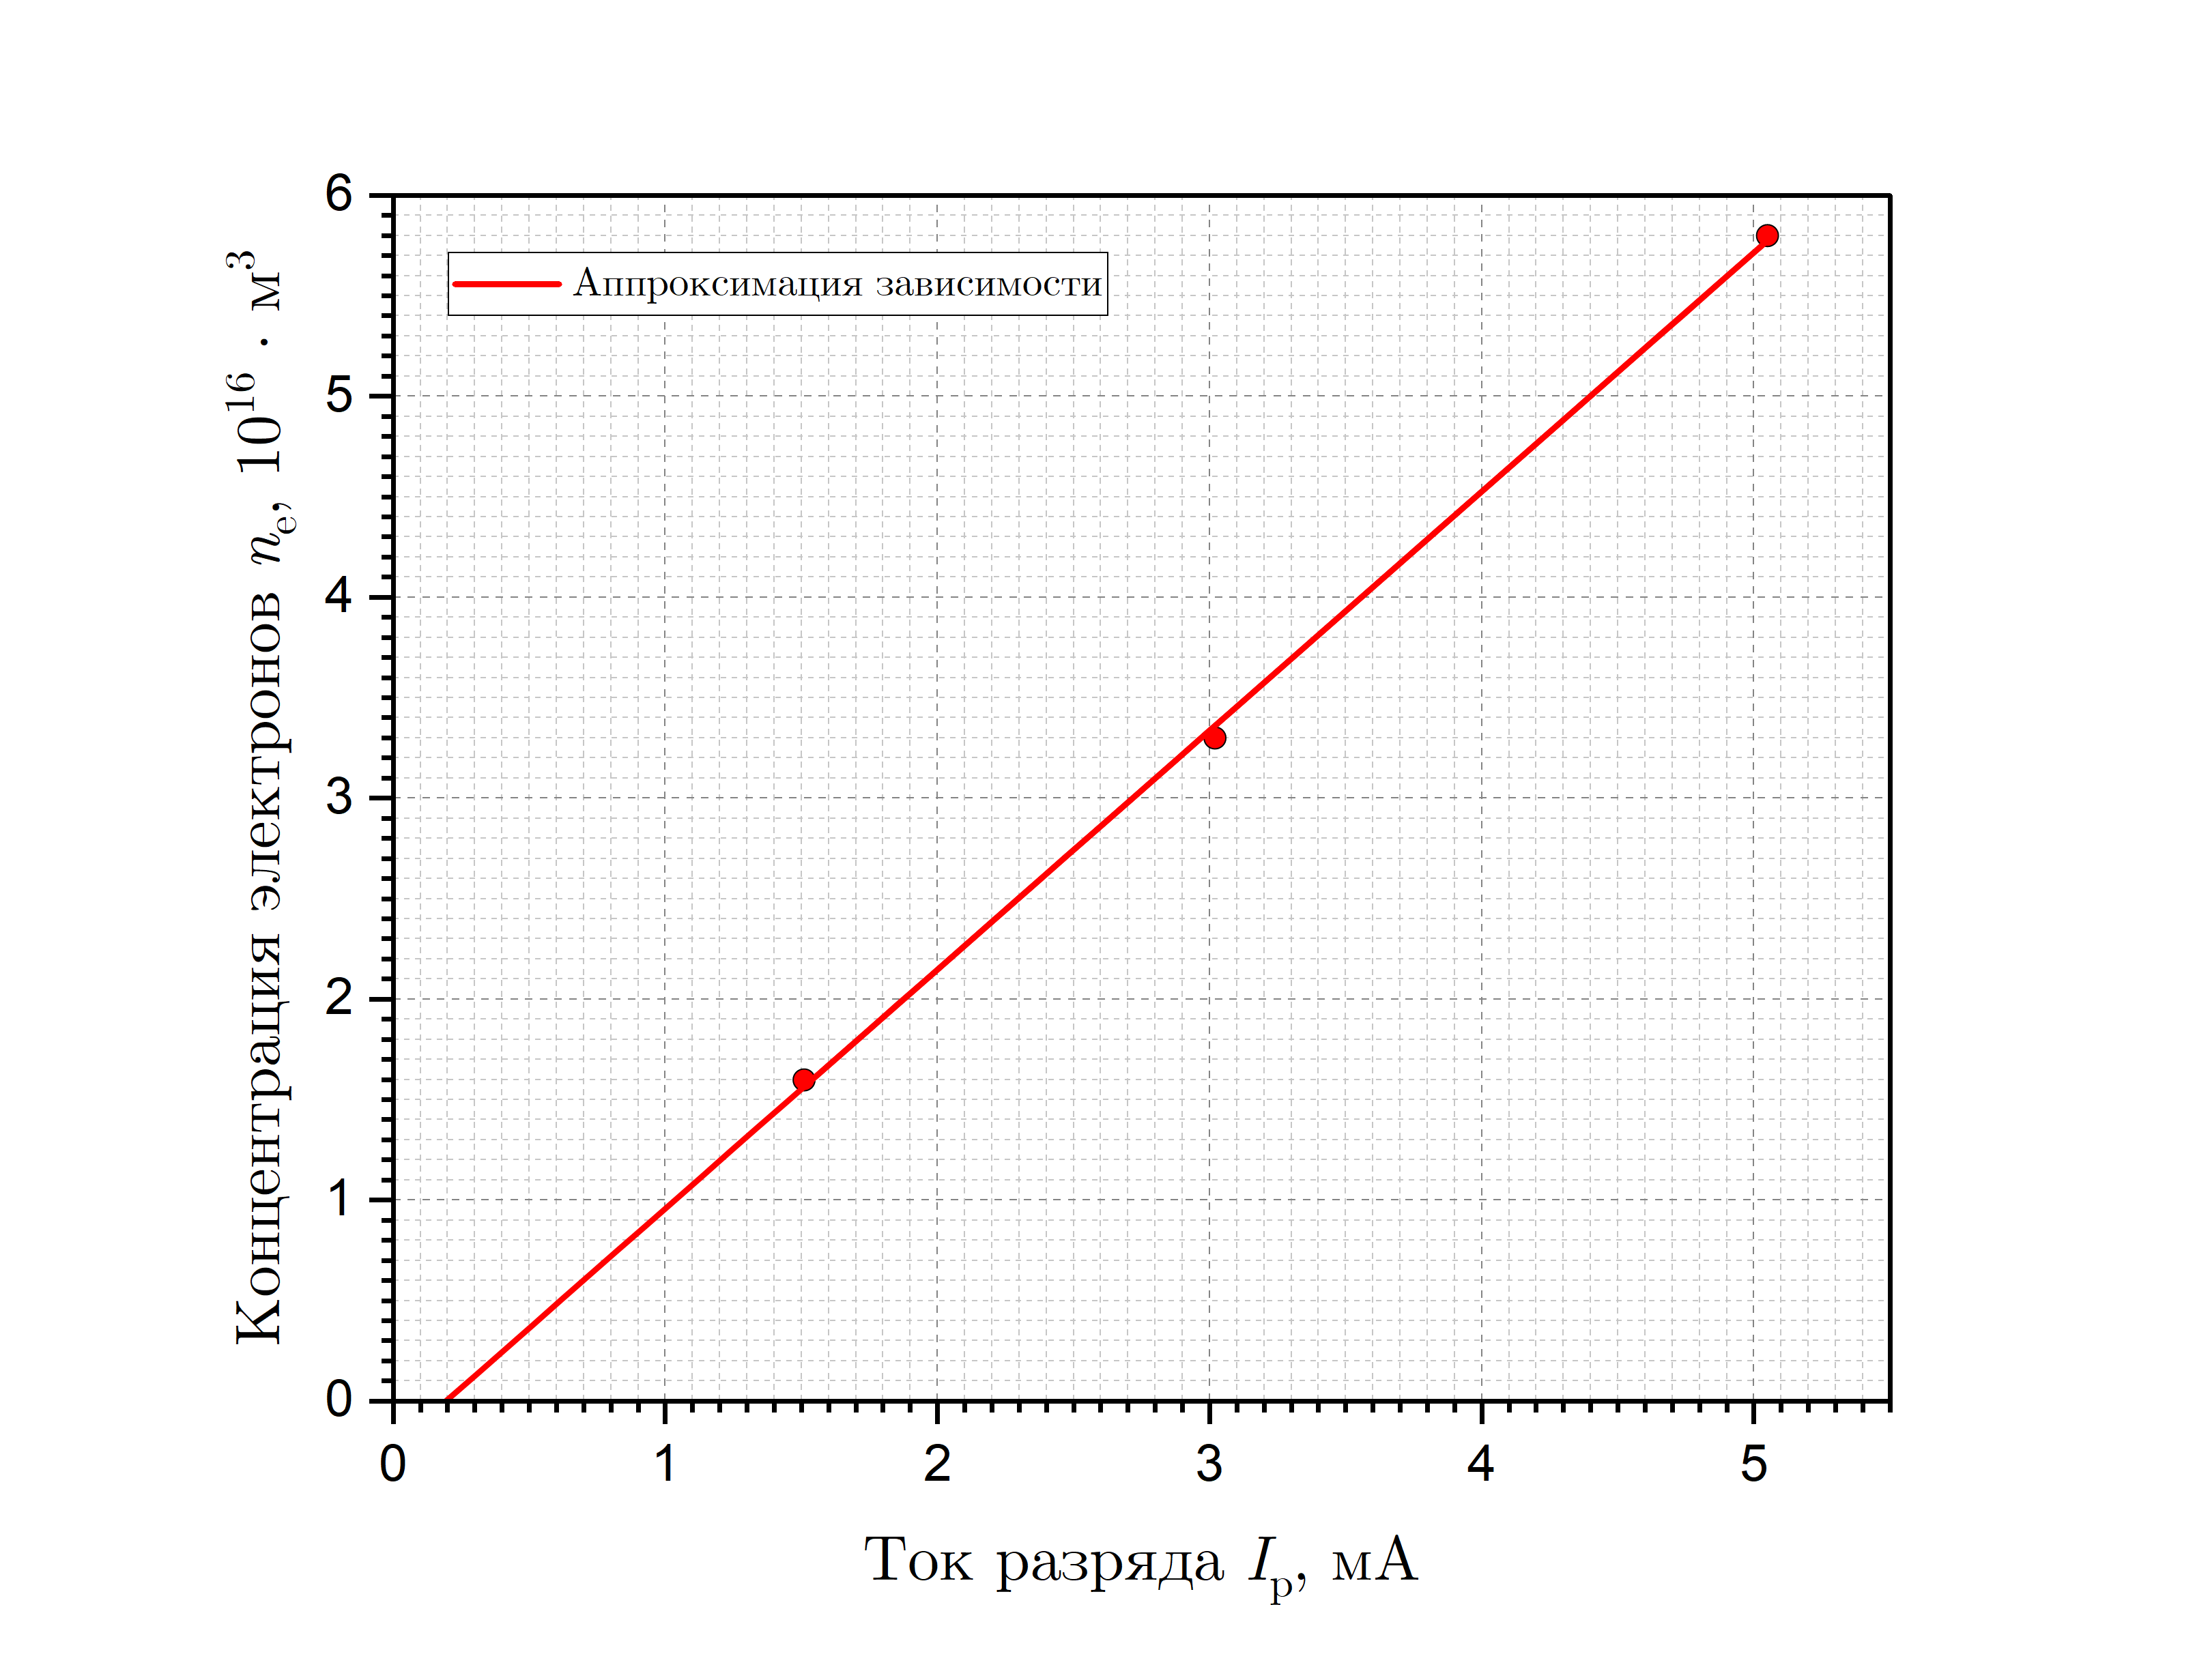
\includegraphics[width = 14 cm]{images/graph_nI.png}
        \caption{Зависимость концентрации электронов $n_e$ от тока разряда $I_{\text{р}}$} 
        \label{graph:conc}
    \end{figure}

    \section{Заключение}

    \begin{enumerate}
        \item В данной работе были изучены вольт-амперная характеристика тлеющего разряда и свойства плазмы методом зондовых характеристик.

        \item В первой части работы были проведены измерения ВАХ разряда, результат успешно сопоставлен участку, соответствующему тлеющему разряду на характерной ВАХ (см. рис. \ref{graph:theor_VAC}).

        \item Во второй части работы были измерены зондовых характеристики плазмы при различных токах разряда. Полученные данные были обработаны, с их помощью было проведено исследование основных параметров плазмы -- температуры и концентрации ионов (см. таблицу \ref{table:results}).

        \item В процессе выполнения работы сделан вывод об \textit{идеальности} и \textit{квазинейтральности} плазмы во всём рабочем диапазоне.

        \item Построены графики зависимости температуры плазмы и концентрации ионов в ней от тока разряда. Заметим, что концентрация с хорошей точностью линейно растёт с увеличением тока, температура, наоборот, растёт нелинейно.
    \end{enumerate}

\end{document}